%% BioMed_Central_Tex_Template_v1.06
%%                                      %
%  bmc_article.tex            ver: 1.06 %
%                                       %

%%IMPORTANT: do not delete the first line of this template
%%It must be present to enable the BMC Submission system to
%%recognise this template!!

%%%%%%%%%%%%%%%%%%%%%%%%%%%%%%%%%%%%%%%%%
%%                                     %%
%%  LaTeX template for BioMed Central  %%
%%     journal article submissions     %%
%%                                     %%
%%          <8 June 2012>              %%
%%                                     %%
%%                                     %%
%%%%%%%%%%%%%%%%%%%%%%%%%%%%%%%%%%%%%%%%%


%%%%%%%%%%%%%%%%%%%%%%%%%%%%%%%%%%%%%%%%%%%%%%%%%%%%%%%%%%%%%%%%%%%%%
%%                                                                 %%
%% For instructions on how to fill out this Tex template           %%
%% document please refer to Readme.html and the instructions for   %%
%% authors page on the biomed central website                      %%
%% http://www.biomedcentral.com/info/authors/                      %%
%%                                                                 %%
%% Please do not use \input{...} to include other tex files.       %%
%% Submit your LaTeX manuscript as one .tex document.              %%
%%                                                                 %%
%% All additional figures and files should be attached             %%
%% separately and not embedded in the \TeX\ document itself.       %%
%%                                                                 %%
%% BioMed Central currently use the MikTex distribution of         %%
%% TeX for Windows) of TeX and LaTeX.  This is available from      %%
%% http://www.miktex.org                                           %%
%%                                                                 %%
%%%%%%%%%%%%%%%%%%%%%%%%%%%%%%%%%%%%%%%%%%%%%%%%%%%%%%%%%%%%%%%%%%%%%

%%% additional documentclass options:
%  [doublespacing]
%  [linenumbers]   - put the line numbers on margins

%%% loading packages, author definitions

%\documentclass[twocolumn]{bmcart}% uncomment this for twocolumn layout and comment line below
\documentclass{bmcart}

%%% Load packages
%\usepackage{amsthm,amsmath}
%\RequirePackage{natbib}
%\RequirePackage[authoryear]{natbib}% uncomment this for author-year bibliography
%\RequirePackage{hyperref}
\usepackage[utf8]{inputenc} %unicode support
\usepackage{graphicx}
%\usepackage[applemac]{inputenc} %applemac support if unicode package fails
%\usepackage[latin1]{inputenc} %UNIX support if unicode package fails


%%%%%%%%%%%%%%%%%%%%%%%%%%%%%%%%%%%%%%%%%%%%%%%%%
%%                                             %%
%%  If you wish to display your graphics for   %%
%%  your own use using includegraphic or       %%
%%  includegraphics, then comment out the      %%
%%  following two lines of code.               %%
%%  NB: These line *must* be included when     %%
%%  submitting to BMC.                         %%
%%  All figure files must be submitted as      %%
%%  separate graphics through the BMC          %%
%%  submission process, not included in the    %%
%%  submitted article.                         %%
%%                                             %%
%%%%%%%%%%%%%%%%%%%%%%%%%%%%%%%%%%%%%%%%%%%%%%%%%


%\def\includegraphic{}
%\def\includegraphics{}



%%% Put your definitions there:
\startlocaldefs
\endlocaldefs


%%% Begin ...
\begin{document}

%%% Start of article front matter
\begin{frontmatter}

\begin{fmbox}
\dochead{Research}

%%%%%%%%%%%%%%%%%%%%%%%%%%%%%%%%%%%%%%%%%%%%%%
%%                                          %%
%% Enter the title of your article here     %%
%%                                          %%
%%%%%%%%%%%%%%%%%%%%%%%%%%%%%%%%%%%%%%%%%%%%%%

\title{Stagnation, deterioration and disparities on adulthood survival in Mexican states, 1990-2015.  }

%%%%%%%%%%%%%%%%%%%%%%%%%%%%%%%%%%%%%%%%%%%%%%
%%                                          %%
%% Enter the authors here                   %%
%%                                          %%
%% Specify information, if available,       %%
%% in the form:                             %%
%%   <key>={<id1>,<id2>}                    %%
%%   <key>=                                 %%
%% Comment or delete the keys which are     %%
%% not used. Repeat \author command as much %%
%% as required.                             %%
%%                                          %%
%%%%%%%%%%%%%%%%%%%%%%%%%%%%%%%%%%%%%%%%%%%%%%

\author[
   addressref={aff1},                   % id's of addresses, e.g. {aff1,aff2}
   corref={aff1},     
   noteref={n1},                  % id of corresponding address, if any
   %noteref={n1},                        % id's of article notes, if any
   email={jmaburto@health.sdu.dk}   % email address
]{\inits{JMA}\fnm{Jos\'e Manuel} \snm{Aburto}}
\author[
   addressref={aff2},
   noteref={n1},
   email={riffe@demogr.mpg.de}
]{\inits{TR}\fnm{Tim} \snm{Riffe}}
\author[
   addressref={aff1},                   % id's of addresses, e.g. {aff1,aff2}
   email={vcanudas@health.sdu.dk}
]{\inits{VCR}\fnm{Vladimir} \snm{Canudas-Romo}}

%%%%%%%%%%%%%%%%%%%%%%%%%%%%%%%%%%%%%%%%%%%%%%
%%                                          %%
%% Enter the authors' addresses here        %%
%%                                          %%
%% Repeat \address commands as much as      %%
%% required.                                %%
%%                                          %%
%%%%%%%%%%%%%%%%%%%%%%%%%%%%%%%%%%%%%%%%%%%%%%

\address[id=aff1]{%                           % unique id
  \orgname{Department of Public Health \& Max Planck Odense Center on the Biodemography of Aging at University of Southern Denmark}, % university, etc
  \street{J.B. Winsl{\o}ws Vej 9},                     %
  \postcode{5000}                                % post or zip code
  \city{Odense},                              % city
  \cny{Denmark}                                    % country
}
\address[id=aff2]{%
  \orgname{Max Planck Institute for Demographic Research},
  \street{ Konrad-Zuse-Stra{\ss}e 1},
  \postcode{18057}
  \city{Rostock},
  \cny{Germany}
}

%%%%%%%%%%%%%%%%%%%%%%%%%%%%%%%%%%%%%%%%%%%%%%
%%                                          %%
%% Enter short notes here                   %%
%%                                          %%
%% Short notes will be after addresses      %%
%% on first page.                           %%
%%                                          %%
%%%%%%%%%%%%%%%%%%%%%%%%%%%%%%%%%%%%%%%%%%%%%%

\begin{artnotes}
%\note{Sample of title note}     % note to the article
\note[id=n1]{Equal contributor} % note, connected to author
\end{artnotes}

\end{fmbox}% comment this for two column layout

%%%%%%%%%%%%%%%%%%%%%%%%%%%%%%%%%%%%%%%%%%%%%%
%%                                          %%
%% The Abstract begins here                 %%
%%                                          %%
%% Please refer to the Instructions for     %%
%% authors on http://www.biomedcentral.com  %%
%% and include the section headings         %%
%% accordingly for your article type.       %%
%%                                          %%
%%%%%%%%%%%%%%%%%%%%%%%%%%%%%%%%%%%%%%%%%%%%%%

\begin{abstractbox}



\begin{abstract} % abstract
\parttitle{Background} The second half of the 20th century was marked by sizable improvements in mortality, living conditions and health in most Latin American countries. In Mexico, these improvements have slowed down recently as a result of opposing trends in particular causes of death. We aim to extend these findings by age groups to the 32 Mexican states by measuring the potential gains in life expectancy due to avoidable causes of death.
\parttitle{Methods} We use mortality data from 1990 to 2015 for all states and calculate temporary life expectancies for three large age groups, and compare these with a low mortality benchmark. We use the concept of avoidable mortality  and use standard decomposition techniques to disentangle age-cause-specific effects on survival.
\parttitle{Results} We find improvements in survival for the population below age 15. However, the adult population aged 15 to 39 shows deterioration among males after 2006 in almost every state as a result of an increase in homicide mortality. Adults aged 40 to 74 show an unexpected decrease in the low mortality benchmark, indicating universal deterioration in both males and females. State-specific departures from this benchmark was caused by ischemic heart diseases, diabetes, cirrhosis and homicide mortality, mainly. We find large health disparities between states, particularly for the adult population and specially after 2005.
\parttitle{Conclusions} Mexico has succeeded in reducing mortality and between-states inequalities in children and the young population. However, the adult population is becoming vulnerable as they have not been able to reduce the burden of conditions amenable to health services and some related to public policies (e.g. homicides). This has led to large health disparities between states in the last 25 years.
%\parttitle{Second part title} %if any
%Text for this section.
\end{abstract}

%%%%%%%%%%%%%%%%%%%%%%%%%%%%%%%%%%%%%%%%%%%%%%
%%                                          %%
%% The keywords begin here                  %%
%%                                          %%
%% Put each keyword in separate \kwd{}.     %%
%%                                          %%
%%%%%%%%%%%%%%%%%%%%%%%%%%%%%%%%%%%%%%%%%%%%%%

%to think about
\begin{keyword}
\kwd{health inequalities}
\kwd{adult health}
\kwd{causes of death}
\kwd{homicides}
\kwd{ischemic heart diseases}
\kwd{diabetes}
\kwd{cirrhosis}
\end{keyword}

% MSC classifications codes, if any
%\begin{keyword}[class=AMS]
%\kwd[Primary ]{}
%\kwd{}
%\kwd[; secondary ]{}
%\end{keyword}

\end{abstractbox}
%
%\end{fmbox}% uncomment this for twcolumn layout

\end{frontmatter}

%%%%%%%%%%%%%%%%%%%%%%%%%%%%%%%%%%%%%%%%%%%%%%
%%                                          %%
%% The Main Body begins here                %%
%%                                          %%
%% Please refer to the instructions for     %%
%% authors on:                              %%
%% http://www.biomedcentral.com/info/authors%%
%% and include the section headings         %%
%% accordingly for your article type.       %%
%%                                          %%
%% See the Results and Discussion section   %%
%% for details on how to create sub-sections%%
%%                                          %%
%% use \cite{...} to cite references        %%
%%  \cite{koon} and                         %%
%%  \cite{oreg,khar,zvai,xjon,schn,pond}    %%
%%  \nocite{smith,marg,hunn,advi,koha,mouse}%%
%%                                          %%
%%%%%%%%%%%%%%%%%%%%%%%%%%%%%%%%%%%%%%%%%%%%%%

%%%%%%%%%%%%%%%%%%%%%%%%% start of article main body
% <put your article body there>

%%%%%%%%%%%%%%%%
%% Background %%

\section*{Background}
The second half of the 20th century was marked by sizable improvements in mortality, living
conditions and health in most Latin American countries \cite{who2000}. 
In Mexico, these improvements have slowed down recently as a result of opposing
trends in particular causes of death. For instance, homicide and diabetes
increased during the first decade of the 2000's, even as infectious and
respiratory diseases continued to fall over the same period. While life
expectancy at birth increased by 4.3 years for males (from 67.6 to 71.9) and 3.4
for females (from 73.8 to 77.2) between 1990 and 2000 \cite{SOMEDE},
between 2000 and 2010, life expectancy at birth entered into a period of
stagnation for males and slowed progress for females \cite{canudas2014}. 


This
period coincides with ongoing public health interventions, such as the Universal Vaccination Program, and with the implementation of Seguro
Popular, which aim to provide primary and secondary
health care to the uninsured population and allocate funds to cover catastrophic
health expenditures \cite{knaul2005}. Further, conditional cash transfer programs were introduced to supply incentives for families to reinvest in education, health, and nutrition in 1997 \cite{neufeld2012}. Some evidence
suggests that Mexico experienced substantial decreases in infant and child
mortality, along with improvements that contributed to the reduction of
mortality and in the prevalence of acute malnutrition between 1980 and 2000
because of these interventions \cite{sepulveda2006}. Similarly, by 2012 Seguro Popular had provided health insurance coverage to an additional 52 million
people in Mexico that previously did not have any access to public health care and, as a result, there has been a reduction in catastrophic health expenditures \cite{knaul2012}.

Conditional cash transfers are focused on the poorest states, and Seguro Popular was introduced at different times in different states. In addition, Mexico faces a rapid aging process in which we can anticipate the interaction between infectious diseases and noncommunicable conditions \cite{Bygbjerg1499} on the adult population.\footnote{The percentage of the population aged 60 or older is projected to go from 10\% in 2015 to 15\% in 2030 \cite{CONAPO}.} Although these actions underscore broad progress in public health interventions, they mask disparities between Mexican states and the epidemiological patterns for different age groups. Therefore, it is necessary to assess the varied impacts that these interventions may have had on mortality in Mexican states \cite{urquieta2015evolution}. 

 
 One approach to approximate the impact of health care and other interventions, and to reveal potential areas of improvement is by operationalizing the
 concept of Avoidable or Amenable Mortality (hereafter abbreviated AM)
 \cite{nolte&mckee2004, nolte&mckee2008,elo2014}. This categorization of mortality aims to measure the quality of health service systems by selecting certain
 causes of death that should not occur in the presence of effective and
 timely health care. Among industrialized countries, such as United States,
 Australia, France, Japan, a reduction in AM rates was
 observed over the past 20 years
 \cite{nolte&mckee2008}. Avoidable mortality rates fell, on average, by 17\%
 for males and 14\% for females in these countries. Despite mortality reductions from cancers and circulatory diseases for
 both sexes, heterogeneity between countries persists, with the United
 States showing the smallest reductions (around 5\%) for both sexes  \cite{nolte&mckee2008}. 
 
 In Mexico, the components of avoidable mortality had different trends since the
late 1990's. Mortality from infectious diseases and nutrition-related conditions decreased between 2000 and 2004 \cite{francomarina2006}, while deaths related to diabetes and circulatory diseases increased in the same period \cite{agudelo2014efecto}. Importantly, increases in the latter causes
of death were concentrated in the poorest states of the country
\cite{davila2014mortalidad}. 

We extend previous analyses by using the most recent available data to study mortality trends by cause of death for all 32 states, by sex, and over the full period from 1990 to 2015. This choice of period covers several public health interventions and captures several major trends in state and cause-of-death variation. We further segment AM into health intervention-related AM and
behavior-related AM causes that capture the epidemiological patterns of Mexico \cite{Aburto2015}. In addition, our work differentiates from earlier studies by comparing state mortality patterns with an easy-to-understand low-mortality benchmark calculated for large age groups (i.e. 0-14, 15-49, 50-84). This concept has been previously used in mortality studies \cite{whelpton1947}, and further developed elsewhere 
\cite{wunsch1975minimum,vallin2008minimum}. Deviations from the low-mortality benchmark indicate a strong potential for improvement.

We hypothesize age-dependent variations in mortality outcomes.
In particular, we expect convergence between states and improvement in survival
for young people, since public health interventions are mainly focused on infant and child health. For instance, the vaccination program and Seguro Popular aim to fully cover children in the entire country, and recent
evidence suggests a decrease in mortality below age 15 due to a decline
in infectious and respiratory diseases \cite{gonzalez2016mexico}. On the contrary, we
expect little improvement in survival for the young-adult population due to the sudden and egregious rise in homicide mortality, and among older adults because of the increase in diabetes along with endocrine/metabolic diseases in these ages in the country \cite{gonzalez2011health,gonzalez2016mexico}. Although every
state has the commitment to provide universal coverage and equitable access to
health care, we anticipate disparities between states
in mortality improvements due to state differences in epidemiological patterns  \cite{gomez2016dissonant} and differences in how  health care programs have been delivered to the population
\cite{Frenk2006}.


\section*{Data \& Methods} 
Our analyses are based on publicly available anonymized datasets. We used microdata death files produced by the
Mexican Statistical Office (INEGI) from 1990 to 2015 \cite{INEGI}. From these data, 
information on causes of death by single age, sex, and state of residence at the
time of death was extracted. Population estimates from 1990 to 2015 came from the Mexican Population Council (CONAPO) \cite{CONAPO}. These estimates adjust for age misstatement, undercounting, and interstate and international migration. Death counts and estimated of the population exposed to risk were used to calculate cause-age-specific death rates by sex and state from 1990 to 2015.

\subsection*{Classification of Causes of Death}
To classify deaths we use the concept of ``Avoidable/Amenable Mortality'' (AM) \cite{nolte&mckee2004, nolte&mckee2008}. We group causes of death into ten categories based on a previous classification  \cite{elo2014} that has recently been adapted to the case of Mexico \cite{Aburto2015}. The first category refers to those conditions that are susceptible to medical intervention, such as infectious and respiratory diseases, and it is labeled ``Causes amenable to medical service''. We separate diabetes, ischemic heart diseases (IHD), HIV/AIDS, lung
cancer, and cirrhosis because these causes are susceptible to both health behavior
and medical service, and because the first two represent major causes of death
in Mexican adults \cite{gomez2016dissonant}. We also separate
homicide, road traffic accidents, and suicide because they have emerged as
leading causes of death among young people, and the first two recently had a sizeable
impact on life expectancy in Mexico \cite{Aburto2015}. Remaining causes were grouped into a single category labeled ``Other causes''. 

Death data was originally classified according to the International Classification of Diseases (ICD), revision 9 for years 1990 to 1997 and revision 10 for 1998 to 2015 (see Additional file 1 Table 1 for details on ICD codes for each category). For the sake of a consistent cause-of-death classification over studied period, we grouped specific causes using codes from a previous study on avoidable mortality in the US \cite{elo2014}. To check the validity of these cause-of-death bridge codes in Mexico, we performed a sensitivity analysis and did not find major ruptures in mortality trends by AM classification (See Additional file 1, Figure 1). Although ill-defined causes represent a small percentage of the total deaths (2\% in 1992 \cite{rivera2002epidemiological}), we decided to leave them in the residual category rather than redistribute over other causes of death. We suspect that ill-defined causes could be related to specific conditions, such as homicides, in Mexico.

We truncate analysis at age 85 because cause of death classification and age reporting are considered to be inaccurate in death registration at older ages. Further, age 85 is higher than both the mean and modal lifespan in Mexico, and most important changes in survival are captured below it. 

%Table~\ref{tab:causes} lists the cause of death categories we use with relative frequencies by sex for the period 1990-2015.

\subsection*{Age Groups}

We calculate life expectancy in three large age groups to capture mortality differences along the lifespan. Life expectancy in each age group simply refers to the average years of life lived between two ages conditional on survival to the lower age bound. The first age group refers to people aged 0-14. This group is likely to represent improvements in causes amenable to medical service (e.g. infectious diseases and conditions of perinatal period) \cite{canudas2014}. The second group, aged 15-49, is used to capture the effect of homicide mortality and external causes historically related to the young-adult mortality hump. This age group had an important impact on changes in state life expectancy in the first decade of the 2000s \cite{Aburto2015}. The third group covers older adults aged 50-84. We focus on adults because they likely represent a vulnerable group due to deterioration in non-communicable diseases and injury-related mortality in recent years \cite{gonzalez2011health,gomez2016dissonant}.

\subsection*{Statistical \& demographic Methods}
We smooth cause-specific death rates over age and time for each
state and sex separately using a 2-d p-spline
to mitigate random variations between ages \cite{GC2012}. We then calculate period life tables up to
age 84 for males and females from 1990 to 2015 following standard demographic methods \cite{HMDMP}. We calculate the temporary life expectancy \cite{arriaga1984} (See Additional file 1 for a technical overview) and estimate cause-specific contributions to the difference between
each state and the low mortality benchmark using
 standard decomposition techniques \cite{horiuchi2008}. Finally, to measure the level of disparities between states over time, we estimate the coefficient of variation and the Gini coefficient on temporary life expectancy within each age-group and year. In addition, we perform a two way ANOVA and post hoc tests to analyze disparities in temporary life expectancy between states and age groups in Mexico. 

\subsection*{Low mortality benchmark}
Our low-mortality benchmark is calculated in the basis of the lowest observed mortality rates by age, cause of death, from among all states for a given sex and year.

The resulting minimum mortality rate schedule has a unique age profile, and it determines our benchmark temporary life expectancy. The minimum mortality schedule can be treated as the best presently achievable mortality assuming perfect diffusion of the best available practices and technologies in Mexico \cite{vallin2008minimum}. This value is a practical reference because it is based neither on a projection of improvements into the future nor on an arbitrary and likely dissimilar population. 


\subsection*{Limitations}
Mortality data from Mexico are
likely to present inaccuracies in cause-of-death classification due to
comorbidities, particularly at older ages \cite{tobias2001}. To mitigate this,
we focus on ages below 85 and grouped causes of death using ICD codes.
Our estimates regarding homicide mortality are likely to be
underestimated due to inaccurate practices regarding counting, reporting,
and due to the large number of missing individuals in Mexico \cite{HRW2011}.

Avoidable mortality should be understood as an indicator of potential
weaknesses with respect to health care and some public health policies and not
as a definitive assessment \cite{nolte&mckee2008}. The amount of deaths that should be considered avoidable within the avoidable classification is not clear \cite{beltran2011avoidable}. For instance, some researchers consider only 50 percent of heart disease mortality to be avoidable \cite{nolte2012amenable, holland2003}. We do not have information to precisely
measure percentages of avoidable mortality within cause groups in Mexico. Nonetheless, the
difference between a given mortality schedule and the best mortality schedule of
the same year can be conceived of as a minimal definition of avoidable
mortality. The benchmark mortality schedule sets a lower bound to how much mortality could have been avoided. Certainly, even the best mortality schedule will contain elements of mortality that
most would consider avoidable. To the extent that the components of the benchmark schedule were indeed
attained somewhere in Mexico, one can view any excess mortality
with respect to the benchmark schedule as avoidable. We believe this perspective improves on the AM concept by giving a directly measurable standard against which to estimate avoidable deaths.

\section*{Results}

\subsection*{Trends in life expectancy for Mexican states by age-groups}

Figure \ref{Fig1} presents life expectancy between two ages (temporary life
expectancy) by state  for three large age groups, young (ages 0-14), young
adults (15-49) and older adults (50-84), over the period 1990-2015. Grey lines
refer to each one of the 32 states; the black lines represent the average over
states; and the blue lines represent the low mortality benchmark. The black line
at the top of each panel indicates the maximum survival in each age group. For
example, the youngest age group has a maximum of 15 livable years, while young
and older adults have up to 35 years conditional on surviving to ages 15 and 50,
respectively. Any gap between a state line and the blue line represents potential additional years of life if mortality were to achieve the low mortality benchmark.

All states show improvements in the youngest age group since 1990, approaching the low mortality benchmark, which itself is very close to maximum survival below age 15. In contrast, southern states such as Puebla, Chiapas and Tabasco have lagged behind in reducing mortality at these ages throughout the entire period. 	

Life expectancy between ages 15 and 49 shows a common shift after 2005 among males in almost every state in Mexico. In 2005, young males in this age group had a temporary life expectancy of 33.9 years averaged over states. By 2010, the number of states below this level had increased from 14 to 23. Chihuahua, Sinaloa and Durango, in the northern region, experienced a substantial mortality shock in 2010 in this age group, and consequently recorded the largest departures from the low mortality benchmark. In 2015, the state average (33.8) had almost recovered to its 2005 level,
Trends for females are closer to the low mortality benchmark.

Among older adults, life expectancy between ages 50 and 84 shows stagnation and deterioration over the entire period of observation. Even the low mortality benchmark exhibits a gradual downward trend, pointing to a generalized mortality increase. Of a maximum of 35 years, females state average life expectancy declined from 28.8 years in 1990 to 28.3 years in 2010. By 2015, this average only managed to recover to 28.6 years. Among males, the average over states decreased from 26.8 in 1990 to 26.3 in 2010, and 26.6 in 2015. As with young adult males, some states experienced a deterioration after 2005, with a minor recovery since 2010.\\

\begin{center}
[Figure \ref{Fig1} about here]
\end{center}

\subsection*{Health disparities between states and age groups}
Figure \ref{Fig2} shows the trends in inequalities between states in Mexico for males in three age groups, as measured by the coefficient of variation (results for the Gini coefficient are reported in Additional file 1, Figure 2). These indicators measure the variation in temporary life expectancy between states within the three age groups. Larger values are related to higher disparities between states. Both indicators are relative and have the property that even if temporary life expectancy refers to different range of ages, e.g. 0-14 and 15-49, the values are still comparable over age groups and time. Trends show mixed patterns of convergence with temporary divergence, and with females in all cases showing less between-state inequality than males over the entire period studied. 

There are important differences in inequality levels and trends between age groups. Since 1990, state inequality in life expectancy in the youngest age group has been decreasing. Among females, young adults show even lower values than the population in the youngest age group (see Additional file 1, Figure 3). However, males show a crossover in the early 2000's, and after 2005 inequality increased. The highest values are observed in the period 2009-2011. By 2015, state inequalities among young adults had decreased substantially, but still remains higher than that of the youngest age group. Older adults show substantially higher inequality than the other age groups over the entire period studied, but also show steady convergence between states. From 2013, both males and females show a potential rise in disparities between states (Additional file 1 Figure 3).  \\

\begin{center}
[Figure \ref{Fig2} about here]
\end{center}


We further performed a two-way ANOVA on temporary life expectancy by state and age-groups controlling by year. There was a statistically significant interaction between the effects of states and age groups [$F=12.25, p < .001$]. There were also significant differences in temporary life expectancy between age groups [$p < .001$] and states [$p < .001$]. Tukey's HSD post hoc tests were carried out. Results show that 71.7\% of 4,560 possible pairs of comparisons were significantly different at the level of $p < .001$. 

To illustrate discordance between age groups, Figure \ref{Fig3} shows the state ranking of the average temporary life expectancy for the years 2010-15 for males in each age group. States at the top show the highest values in temporary life expectancy, while states in the bottom refer to the lowest values. We chose to highlight the states with most discordant ages. Green and purple lines refer to selected states that show drastic changes in the ranking between different age groups. For example, Sinaloa, in the northern part of Mexico, holds the record life expectancy below age 15; however, young adults (15-49) show one of the lowest values, while older adults are in the sixth position out of 32. Similar trajectories are shown with green lines for Nayarit and Michoac\'an in the central region, Zacatecas in the North, as well as Morelos and Guerrero from the southern region. Conversely, the pattern of age discordance in Hidalgo, Quer\'etaro and Mexico City from the central region, and Yucatan and Puebla in the South (purple lines) is summarized by changing from a lower rank in the youngest age group to a higher one in young adults, followed by lower rank in older adults. \\

\begin{center}
[Figure \ref{Fig3} about here]
\end{center}


\subsection*{Cause-decomposition analysis}


In Figures \ref{Fig4} and \ref{Fig5}, the Mexican states in each region are arranged according to the largest gap with the low mortality benchmark among older adult males in 2015. Figure \ref{Fig4} shows how causes amenable to medical service, diabetes, ischemic heart diseases (IHD), lung cancer, cirrhosis, homicide and road traffic accidents contributed to the gap between each state and the low mortality benchmark from 1990 to 2015 for male older adults (ages 40-84). These are the causes of death that contributed the most to holding states back from achieving the low mortality benchmark. Light-yellow colors indicate negligible contributions, which means that are very close to the low mortality benchmark within each category. Darker red hues indicate larger contributions to the gap. If a particular state is improving during the period, it shows a transition from red to light-yellow. 

Medically amenable causes of death show gradual improvements in most states from 1990 to 2015, bringing them closer to the benchmark in this category. However, large disparities between states and potential for improvements remain. For example, Baja California, Sonora, Chihuahua and Coahuila from the northern region show substantial contributions to the gap. Diabetes mortality has increasingly contributed to widening the benchmark gap in several states, including Coahuila and Tamaulipas in the North, Mexico City, Guanajuato, Mexico state and Tlaxcala in the central region, and Puebla, Veracruz and Tabasco in the South. Similarly, IHD significantly affects the northern part of the country, while cirrhosis is mostly concentrated in the South. Lung cancer and road traffic accidents have lower contributions to the benchmark gap, but these remain important causes of death. Homicides increased the gap in this age group in some states after 2005, such as Chihuahua, Durango and Sinaloa in the North, Colima, Michoacan and Nayarit in the central region, and Guerrero in the South.

\begin{center}
[Figure \ref{Fig4} about here]
\end{center}

Causes amenable to medical service, diabetes, and IHD contributed the largest share to the gap with the low mortality benchmark among older adult females (see Additional file 1, Figure 3). Although almost every state shows improvements in medically amenable causes, these conditions still show potential for further gains in life expectancy. Diabetes shows deterioration in recent years in several states, such as Coahuila, Tamaulipas in the North, Guanajuato and Tlaxcala in the central region, and Puebla, Veracruz, and Tabasco in the South. In the North, IHD did not improve notably from 1990 to 2015 among females in the older adult age group.

In the youngest age group, improvements in life expectancy and in reducing the gap with the low mortality benchmark were mainly driven by causes amenable to medical service among both females and males.  (see Additional file 1, Figures 4 and 5). Finally, homicide mortality and road traffic accidents are the main drivers of the gap with the benchmark among young male adults (ages 15-49) (see Additional file 1, Figures 6 and 7). Homicides contributed more than 2.5 years to the gap with the low mortality benchmark in 2010 in Chihuahua. Other states in the North, including Baja California, Coahuila, Tamaulipas, Nuevo Le\'on, Durango, and Sinaloa experienced substantial increases in homicide after 2005. Similar patterns are also seen in Guerrero and Morelos in the South, and Colima and Nayarit in the central region. The impact of the remaining AM categories in ages 0-14 and 15-49 is negligible. \\

\subsection*{Potential gains and causes of death in 2015}

Figure \ref{Fig5} breaks down the state-specific low mortality benchmark gap for males aged 50-84 into potential gains and their cause of death composition. The left panel shows the potential gains for older adults if the low mortality benchmark were achieved in 2015 (Results for previous years and other age groups are shown in the Additional file 1). The right panel shows the proportion of potential gains due to specific causes of death in 2015.

Every state in Mexico could increase survival by at least one year in older adult ages if they were to achieve the low mortality benchmark. However, for 17 of them the gap with the benchmark is higher than 2 years, and for 3 states in the northern region it is greater than 3 years. In females, with the exception of Sinaloa and Nayarit, all the states show the potential to gain over an additional year of life between ages 50-84 (see Additional file 1, Figure 9). %Since 2005, no major improvements were observed, and in some states the potential gains even increased in 2015 compared to 2010, for example San Luis Potos\'i and Zacatecas in the north; Colima, Guanajuato, Mexico City in the central region; and all the southern region, with the exception of Guerrero. 

More than half of these potential gains in life expectancy between ages 50 and 84 are due to avoidable causes of death in every state of Mexico (right panel), and in more than 60\% of the states these causes account for more than 75\% of potential years won. The three main causes of death accounting for these differences are conditions amenable to medical service (AMS) (green), diabetes (beige) and IHD (purple). This is true also for females (see Additional file 1, Figure 10). Cirrhosis explains a considerable proportion of the gap mainly in states in the central and southern regions. Homicide mortality is present in almost every state, particularly in Guerrero, Morelos in the South, Nayarit and Colima in the central region, and Sinaloa in the North. Among young adult males (ages 15-49), homicide mortality is still the main cause of death behind the benchmark mortality gap in most states. The effect is concentrated in the northern states and some states in the South, such as Morelos and Guerrero.

\begin{center}
[Figure \ref{Fig5} about here]
\end{center}



\section*{Discussion}
%Most important messages from the paper: health disparities, over states and ages. The worsening mortality in adults, the impact of homicide, diabetes, IHD and cirrhosis
In Mexico since 1990, life expectancy in three large age groups has followed discordant patterns of rise, deterioration, and stagnation. Such patterns have been driven mainly by causes of death that are amenable to medical service (such as infectious and respiratory diseases) and health behaviors (such as homicides, diabetes, IHD, and cirrhosis). Patterns in these two large cause-ofdeath categories led to contrasting levels of inequality in the country. Our research disentangles these patterns by measuring the impact of medically amenable mortality and behavior-related mortality on life expectancy relative to a low mortality benchmark in three large age groups. %for the youngest ages (below age 15), young adults (15-49) and older adults (50-84) for the 32 Mexican states.

Life expectancy below age 15 converged towards the low mortality benchmark and maximum survival in all 32 Mexican states. These results underscore public health interventions made in the youth population. This is supported by evidence that vaccination coverage has been achieved for the entire young population, and that health insurance coverage has improved, due to vaccination programs and the implementation of Seguro Popular, respectively \cite{urquieta2015evolution}. Causes amenable to medical service are at the heart of such improvements, consisting of decreases in infectious and respiratory diseases associated with public health interventions targeting children \cite{sepulveda2006}. For example, Puebla and Tlaxcala, the states with the lowest life expectancy below age 15 in 1990, improved by more than half a year since the 1990's. Moreover, the average over states improved from 14.5 in 1990 to 14.8 in 2015, with no state below 14.7. As a result of continuous and universal convergence towards the low mortality benchmark, inequalities between states in life expectancy below age 15 have been reduced. 

Opposing the optimistic trend in the under-15 population, increases in homicide mortality reversed gains in male life expectancy, particularly between ages 15-49. These results are consistent with previous studies quantifying the effect of homicide mortality on the stagnation of national life expectancy at birth in the first decade of the 21st century \cite{canudas2014}, and with the reversal experienced in life expectancy in most states between 2005 and 2010 associated with specific public policies \cite{Aburto2015}. Our results extend such findings by adding five years of data and segmenting by specific age groups. We found that after ten years of the unexpected rise in homicide mortality, most states have experienced a slow and partial recovery since 2010. However, the impact of homicide is still higher than the levels observed in 2005. Between 2010 and 2015, this cause of death accounted for most of the gap between states and the low mortality benchmark in ages 15-49. For this age group, the states that show the greatest benchmark gap for homicide in 2015 are Guerrero in the South, and Sinaloa and Chihuahua in the North, which could gain one year, and half a year (each) respectively if homicides were reduced to the level of Yucat\'an, which in this case makes up 100\% of the benchmark. Importantly, these figures are likely to be underestimates caused by under-registration and miss-classification of homicides and missing individuals, particularly in Guerrero \cite{HRW2011,wright2017epistemological}. Moreover, health inequalities in life expectancy between states followed the rise in homicides after 2005 (Figure~\ref{Fig2}), and the considerable discordance between age-groups (Figure~\ref{Fig3}) was likely due in great part to homicide mortality in ages 15-49.
Beyond mortality implications of the rise in homicide, violence has had a toll on perceived vulnerability in the country. As a consequence, women are expected to live over 70\% of their remaining life at age 20 with fear if the perception of vulnerability remains at the 2014 level in Mexico \cite{canudas2017Mexico}. The recent increase in homicides in some states could trigger an increase in the perception of vulnerability, which would result in a higher average lifetime fear in specific states. Although we are not able to link the trends in mortality among young adults in Mexico with specific public policies, some evidence suggests that the propagation of homicide mortality is not only a result of the war between drug cartels, but also because of the implementation of specific policies aimed to mitigate drug cartel operations after 2006 \cite{espinal2015analysis}.
There is no simple way to lessen the impact of homicide mortality, but it is clear that the government has not been able to reduce its burden back to levels observed before 2005.

The population aged 50-84 shows the largest low mortality benchmark gap among both females and males. Out of 35 livable years in this agr group, females lived on average 28.6 years and males 26.5 in 2015 without any clear improvement in the 26 years since 1990. Even the low mortality benchmark shows a downward trend for males and stagnation for females (Figure~\ref{Fig1}). Moreover, this age group exhibits the highest inequality between states in the last 26 years. Our results show that causes of death holding states back from the low mortality benchmark vary between regions. Causes amenable to medical service showed gradual improvements in almost every state since 1990. However, in some states of the northern region such as Baja California, Sonora, and Chihuahua, these causes of death still show large room for improvements among older adults. Diabetes, Ischemic Heart Diseases (IHD) and cirrhosis account for the majority of the gap with the benchmark mortality with large regional differences. For example, IHD is mostly concentrated in the North (Figure \ref{Fig4}), while cirrhosis and diabetes show a stronger impact in the central and southern regions. These results are supported by previous evidence documenting an increase in adult mortality rates from chronic kidney disease, diabetes and cirrhosis since 2000 \cite{gomez2016dissonant}. Lung cancer and homicides had a lower impact on life expectancy for this age group, and both are higher in the northern part of the country. 

The fact that in 2015 the older adult population of Mexico could add more than one year of life in every state for males, and 30 states for females by acheiving the benchmark, underscores vulnerability in these ages. Public health interventions targeting specific causes of death for this age group according to the epidemiological profile of each state, would not only increase life expectancy, but also it would forge a path towards more equality between states in health outcomes. More than 50\% of the potential gains in life expectancy between ages 50 and 84 are due to avoidable mortality, and to a large extent mortality related to health behaviors. For instance, obesity and overweight, risk factors for diabetes and IHD, have dramatically increased since the 1990s in developing countries because of the consumption of cheap, energy-dense food and reduced physical activities \cite{hossain2007obesity}. In this sense, Mexico, along with the USA, has the highest rates of overweight and obesity among all OECD countries  \cite{gonzalez2016mexico} and one of the highest in Latin America, along with Chile, El Salvador, Honduras, and Parguay \cite{aschner2016obesity}. However, obesity prevalence is not homogeneous across Mexico. The highest rates of obesity are concentrated in the northern and central regions \cite{gonzalez2016mexico} and in urban areas of the country \cite{kuri2009prevalence}, which roughly matches our regional pattern of IHD and diabetes mortality.


% add a healthcare utilization and a diffusion hypothesis paragraph, namely, what can be done with the cause-specific, age-specific benchmark gap information?	

\subsection*{Conclusion}
%These findings underscore the need for effective interventions to reduce homicide mortality, as it still contributes the most to survival shortcomings among the young-adult population and mortality inequality among states. Even ten years after the national security strategy that aimed at reducing drug cartels' operations started and homicides begun to spread all over the country \cite{espinal2015analysis}, the effect of homicide on average survival is appalling.

%Improving health is a priority for governments of many developing countries. In part to reduce child mortality, improve maternal health and lessen the impact of other infectious diseases, such as HIV/AIDS, to achieve the Millennium Development Goals established for 2015 \cite{united2009millennium}.  Mexico has succeeded in reducing mortality and inequalities in children and the young population. Nevertheless, our results show that older adults are becoming a vulnerable group, and more efforts are required to reduce the burden of conditions amenable to health services and policy-related conditions. In particular, this group lacks comprehensive interventions to reduce the burden of violence through homicides, chronic-degenerative causes of death, such as diabetes and IHD, and behavior-related conditions such as cirrhosis.  

%There is no simple way to lessen the impact of such conditions, but it is clear that new approaches are needed to improve survival in the adulthood and to minimize health disparities between states. Preventing diabetes and IHD implies fundamental political challenges. Therefore,  public health initiatives should focus in health care for chronic conditions as recently suggested by \cite{knaul2015achieving}, but they should also influence the population towards improving health behavior. Our results reinforce the need of such, among others public health interventions, with an special focus on older adults in the Mexico. 

%\nocite{oreg,schn,pond,smith,marg,hunn,advi,koha,mouse}

%%%%%%%%%%%%%%%%%%%%%%%%%%%%%%%%%%%%%%%%%%%%%%
%%                                          %%
%% Backmatter begins here                   %%
%%                                          %%
%%%%%%%%%%%%%%%%%%%%%%%%%%%%%%%%%%%%%%%%%%%%%%

\begin{backmatter}

\section*{Competing interests}
  The authors declare that they have no competing interests.

\section*{Author's contributions}
TR and JMA conceived the study and performed the demographic and statistical analyses. All authors contributed interpretts. JMA and TR drafted the manuscript, and VCR contributed to revising the manuscript. All authors approved of the final version.
 
\section*{Acknowledgements}
The authors thank their supporting institutions, the European Doctoral School of Demography at Sapienza University, and grants... . The authors also express gratitude to Shammi Luhar for comments on an earlier version of this manuscript.
%%%%%%%%%%%%%%%%%%%%%%%%%%%%%%%%%%%%%%%%%%%%%%%%%%%%%%%%%%%%%
%%                  The Bibliography                       %%
%%                                                         %%
%%  Bmc_mathpys.bst  will be used to                       %%
%%  create a .BBL file for submission.                     %%
%%  After submission of the .TEX file,                     %%
%%  you will be prompted to submit your .BBL file.         %%
%%                                                         %%
%%                                                         %%
%%  Note that the displayed Bibliography will not          %%
%%  necessarily be rendered by Latex exactly as specified  %%
%%  in the online Instructions for Authors.                %%
%%                                                         %%
%%%%%%%%%%%%%%%%%%%%%%%%%%%%%%%%%%%%%%%%%%%%%%%%%%%%%%%%%%%%%

% if your bibliography is in bibtex format, use those commands:
\bibliographystyle{bmc-mathphys} % Style BST file (bmc-mathphys, vancouver, spbasic).
\bibliography{AburtoRiffe_Bib}      % Bibliography file (usually '*.bib' )
% for author-year bibliography (bmc-mathphys or spbasic)
% a) write to bib file (bmc-mathphys only)
% @settings{label, options="nameyear"}
% b) uncomment next line
%\nocite{label}

% or include bibliography directly:
% \begin{thebibliography}
% \bibitem{b1}
% \end{thebibliography}

%%%%%%%%%%%%%%%%%%%%%%%%%%%%%%%%%%%
%%                               %%
%% Figures                       %%
%%                               %%
%% NB: this is for captions and  %%
%% Titles. All graphics must be  %%
%% submitted separately and NOT  %%
%% included in the Tex document  %%
%%                               %%
%%%%%%%%%%%%%%%%%%%%%%%%%%%%%%%%%%%

%%
%% Do not use \listoffigures as most will included as separate files

\section*{Figures}

\begin{figure}[h!]
\centering
\caption{Life expectancy for three age groups, the youngest (0-14), young adults (14-49), and older adults (50-84) by sex for the period 1990-2015.}
\label{Fig1}

%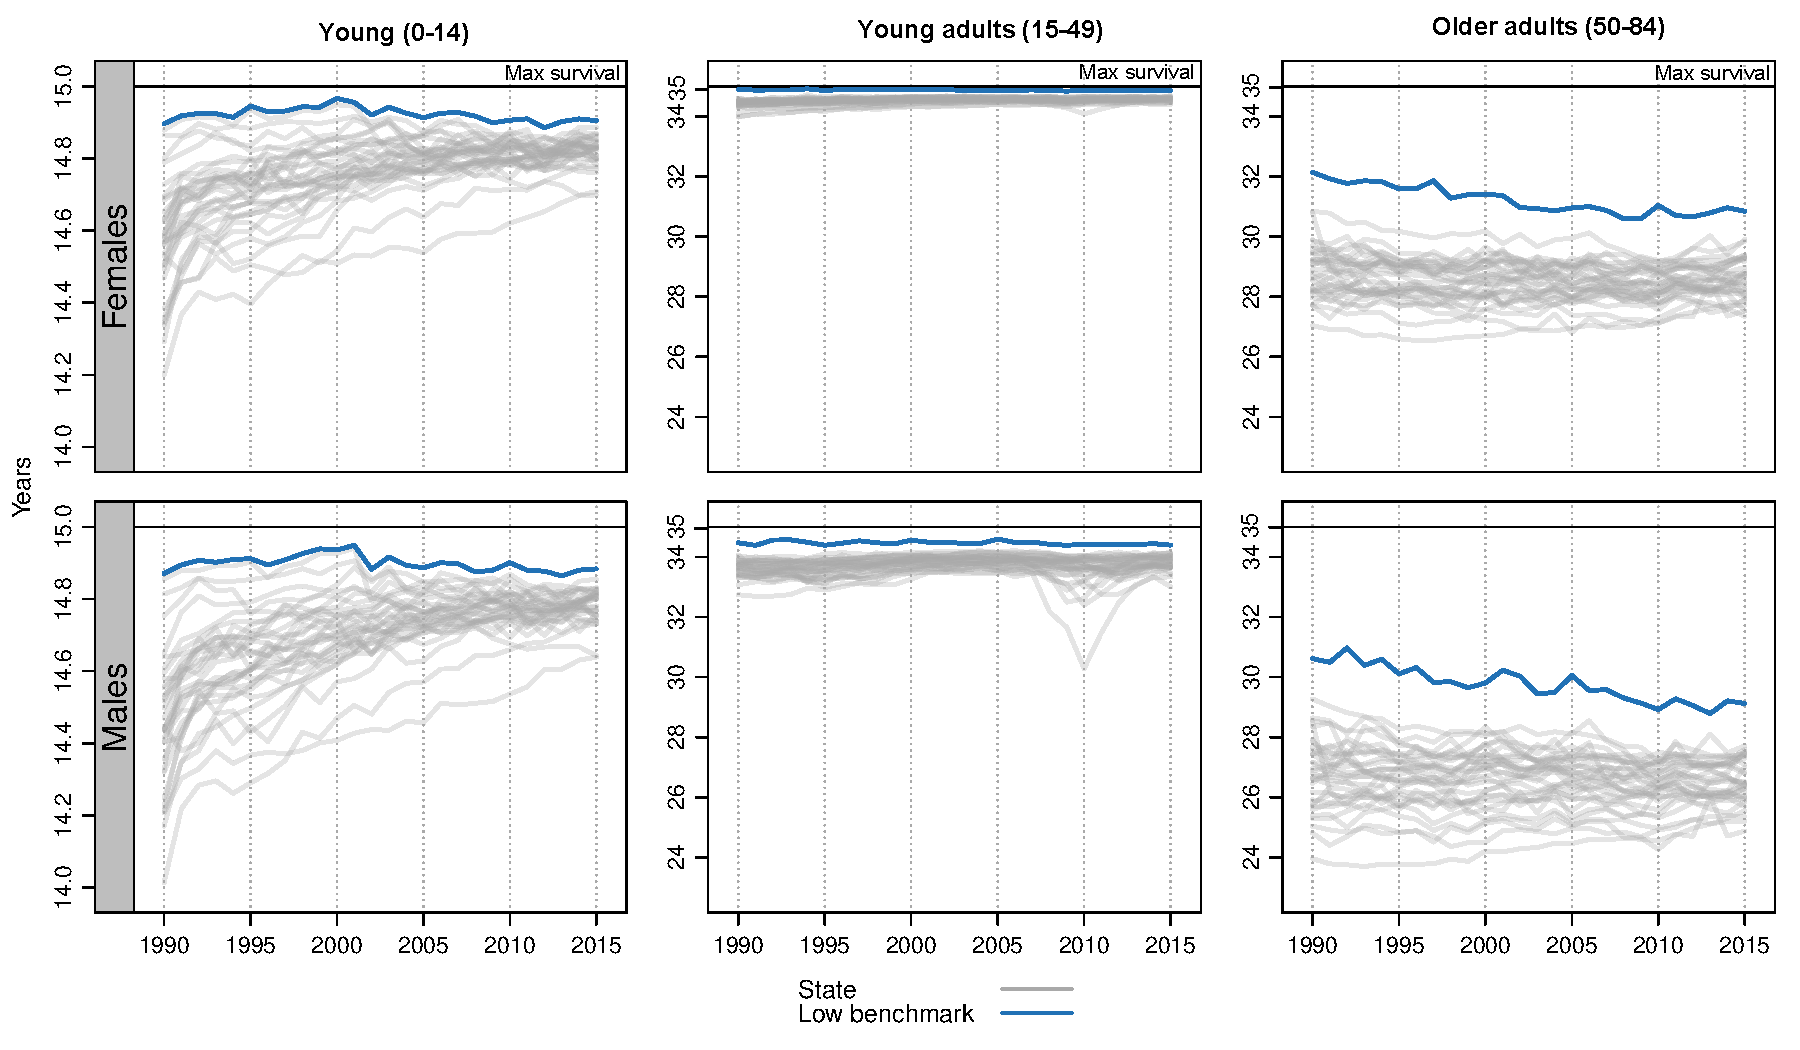
\includegraphics[scale=.35]{Figure1_1.pdf}
Note: Y-axis are not in the same scale in order to capture major trends over the period. Source: calculations based on INEGI and CONAPO files. 
\end{figure}



\begin{figure}[h!]
\centering
\caption{Inequality in male life expectancy between states for young (0-14), young adults (15-49) and older adults (50-84), 1990-2015.}
\label{Fig2}
%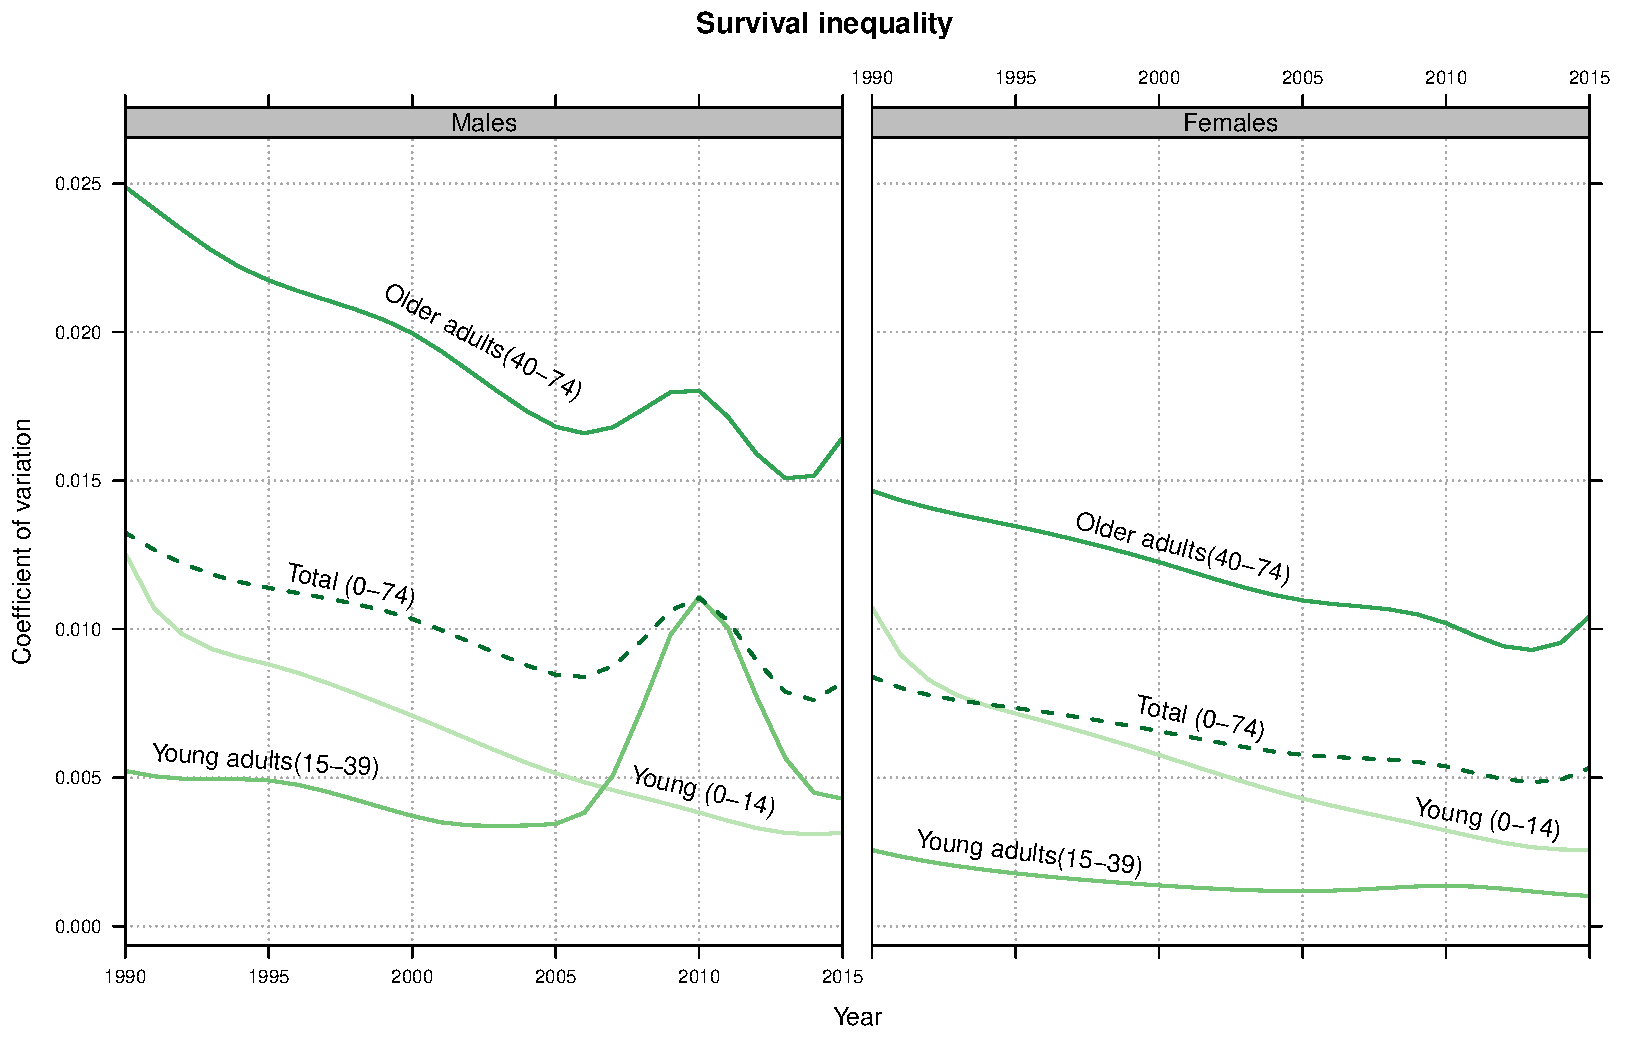
\includegraphics[scale=.4]{CVfig_1.pdf}

Source: calculations based on INEGI and CONAPO files. 
\end{figure}

\begin{figure}[h!]
\centering
\caption{State ranking for average male life expectancy 2010-15 for the youngest (0-14), young adults (14-49), and older adults (50-84).}
\label{Fig3}
%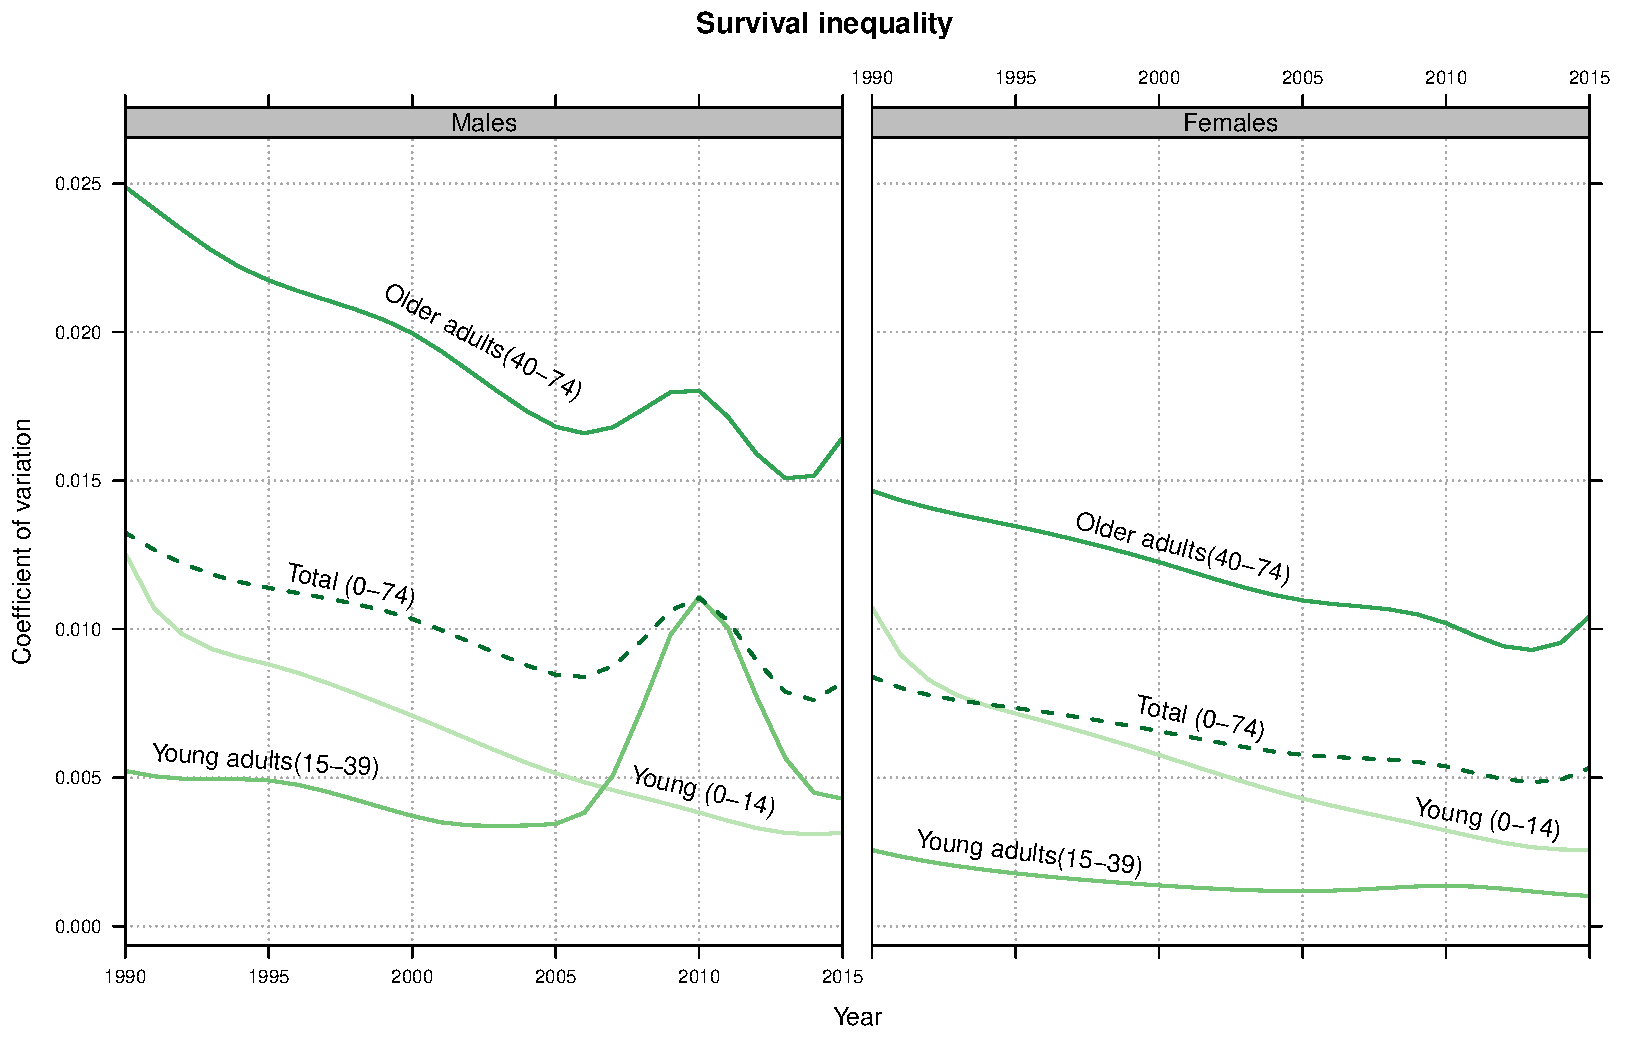
\includegraphics[scale=.4]{CVfig_1.pdf}
Source: calculations based on INEGI and CONAPO files. 
\end{figure}



\begin{figure}[h!]
\centering
\caption{Cause-specific contributions to the gap between states and low mortality benchmark for older male adults (50-84), 1990-2015.}
\label{Fig4}

%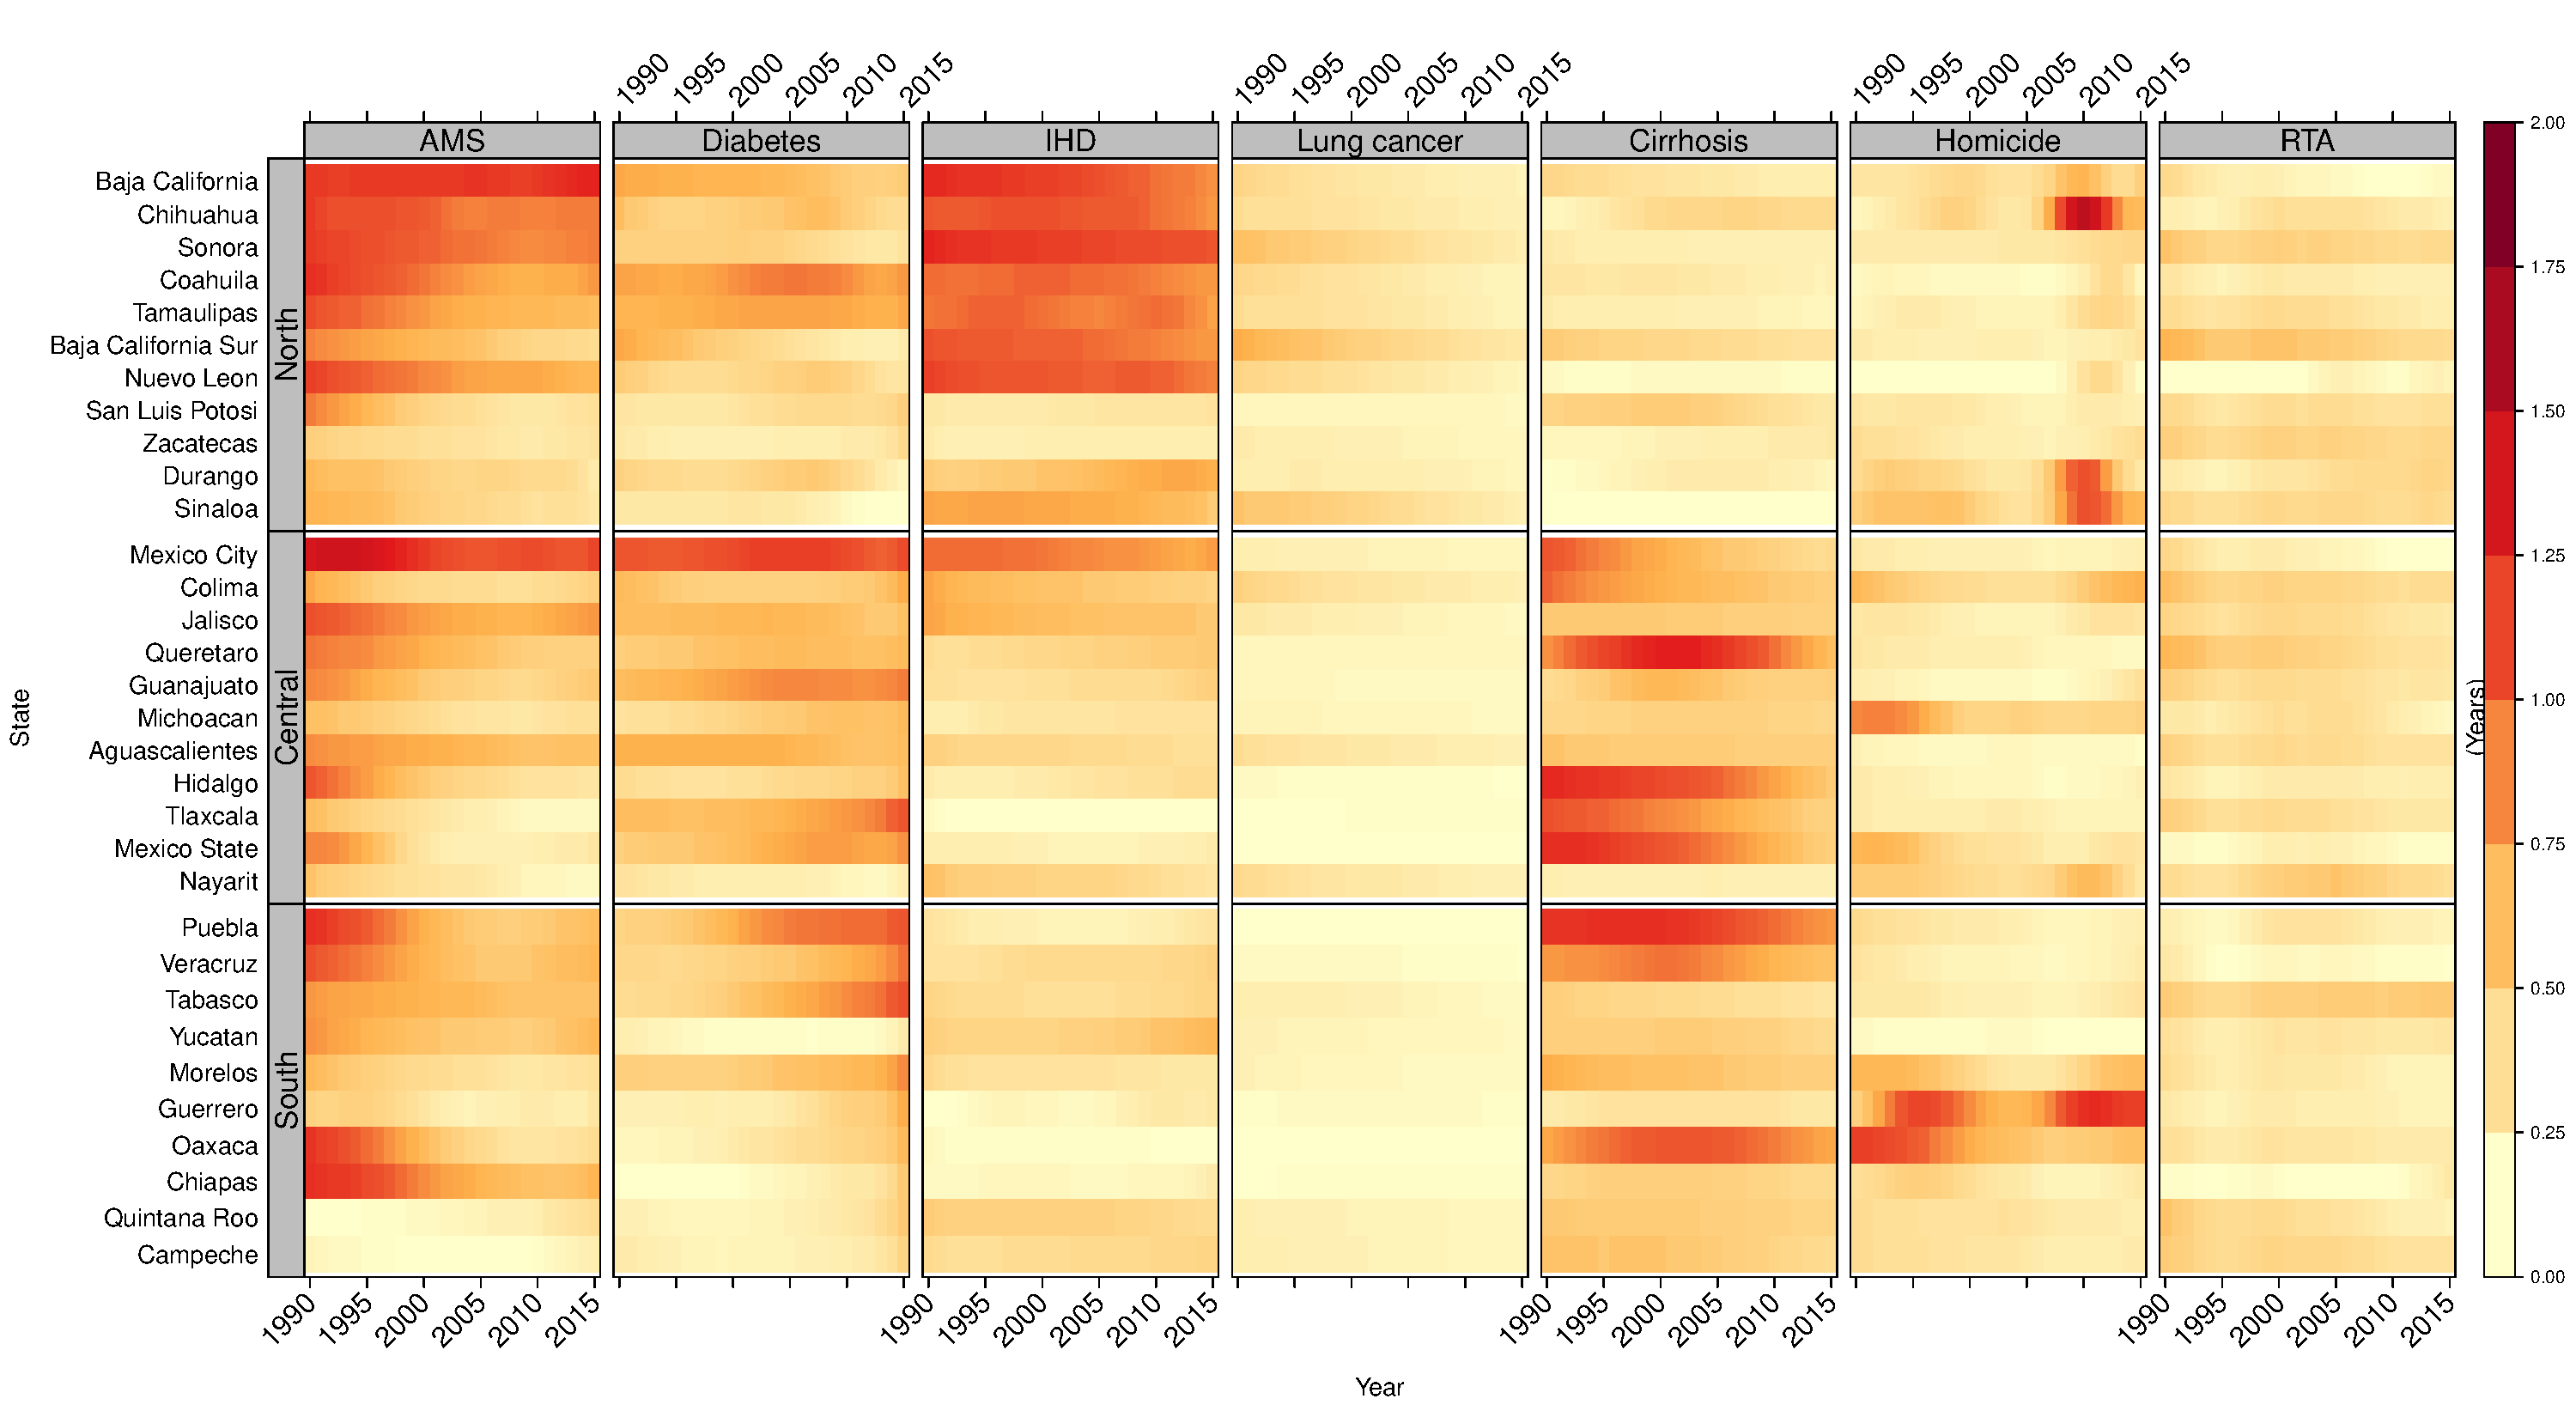
\includegraphics[scale=.23]{AdultMaleheatmap.pdf}
Source: calculations based on INEGI and CONAPO files. 
\end{figure}


\begin{figure}[h!]
\centering
\caption{State specific gap with the low mortality benchmark and its cause-of-death composition for older male adults (50-84) in 2015.}

\label{Fig5}
%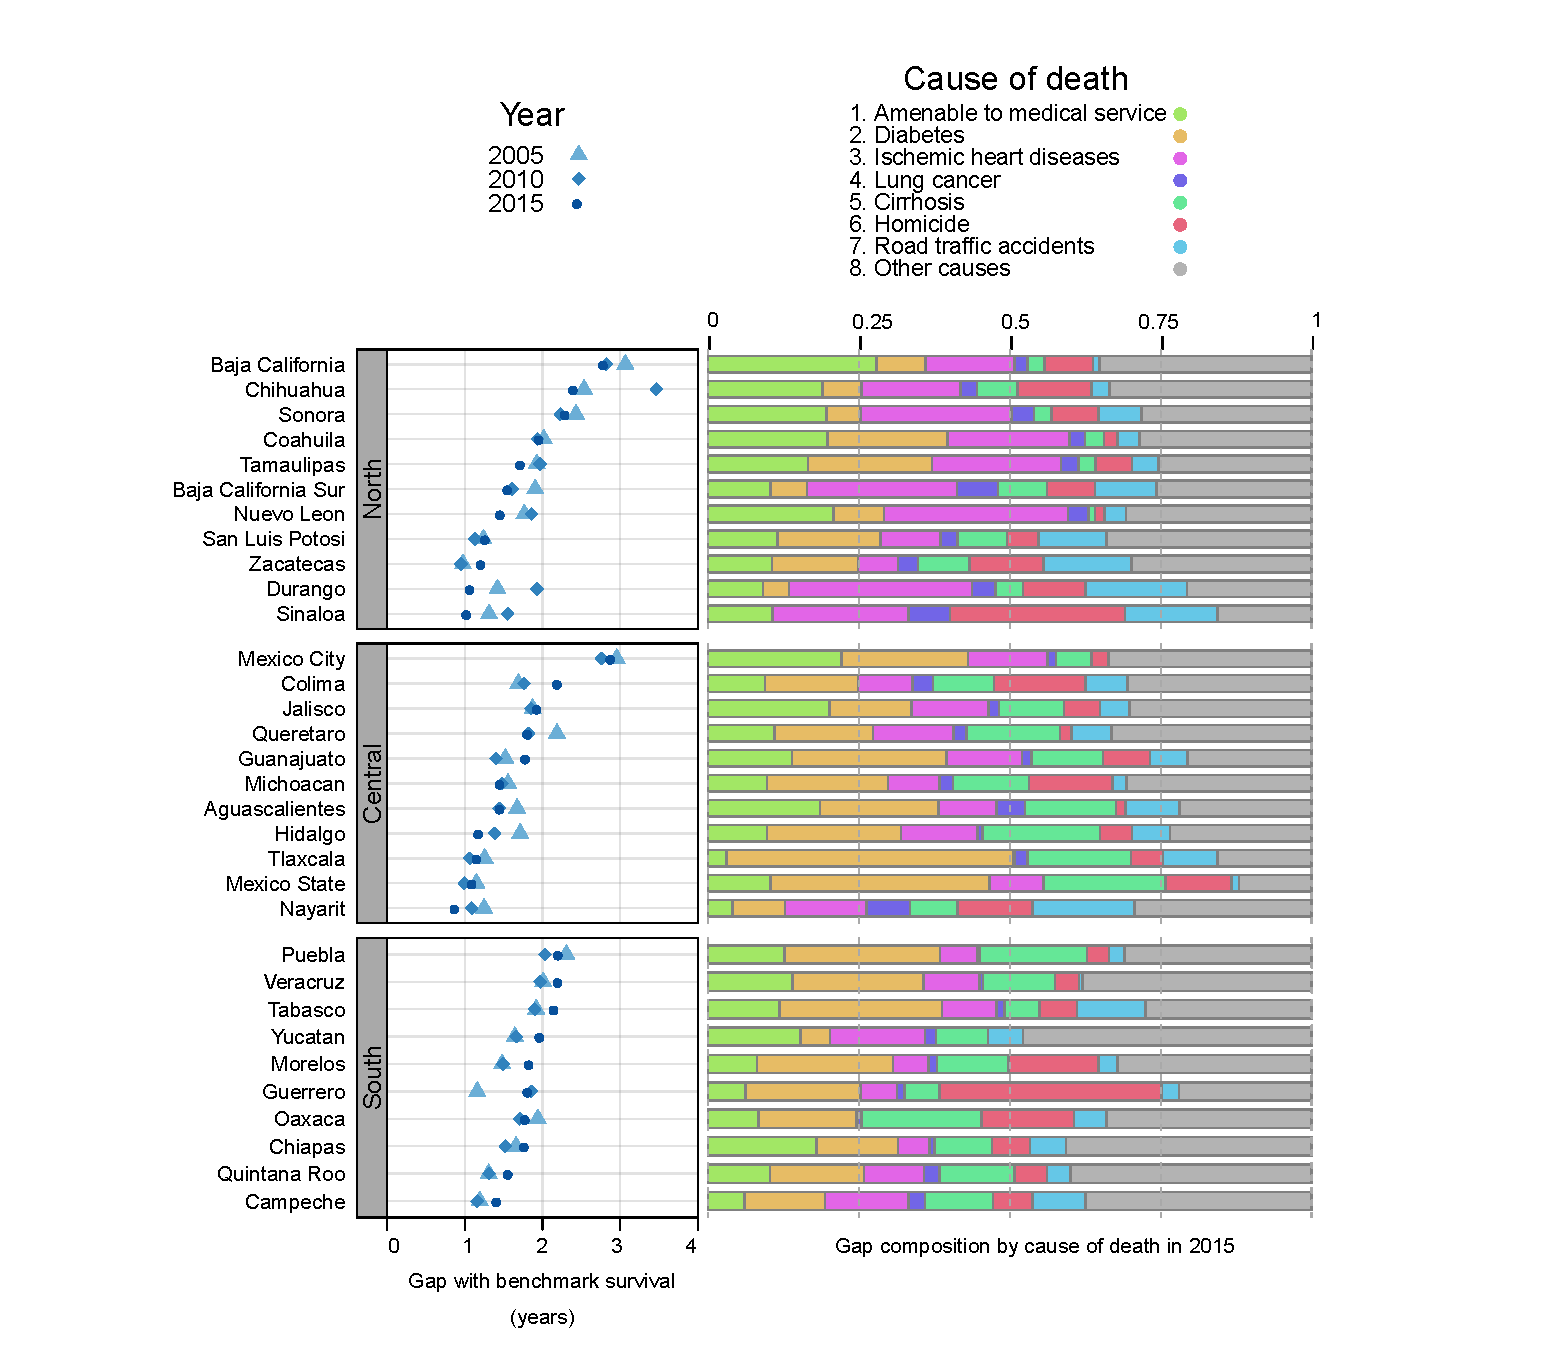
\includegraphics[scale=.45]{Figure_4v2.pdf}

Source: calculations based on INEGI and CONAPO files. 
\end{figure}

%%%%%%%%%%%%%%%%%%%%%%%%%%%%%%%%%%%
%%                               %%
%% Tables                        %%
%%                               %%
%%%%%%%%%%%%%%%%%%%%%%%%%%%%%%%%%%%

%% Use of \listoftables is discouraged.
%%
%\section*{Tables}
% latex table generated in R 3.3.1 by xtable 1.8-2 package
% Wed Jan 18 14:53:15 2017
%\begin{table}[ht]
%\centering
%\caption{Avoidable Mortality classification, 
%             with crude percentages below age 75, years 1990-2015. Source: INEGI files.} 
%\label{tab:causes}
%\begin{tabular}{llllll}
%  \hline
%& Category &\% & Males &  \% & Females \\ 
% &&& (1,000's) & & (1,000's)\\ 
%  \hline
%1&  Causes amenable to medical service & 30.9 \% & 127.5 & 28.2 \% & 114.4 \\ 
%2&  Diabetes & 4.5 \% & 18.7 & 4.9 \% & 19.9 \\ 
%3&  Ischemic heart diseases & 4 \% & 16.4 & 4.2 \% & 17 \\ 
%4&  HIV/AIDS & 0.4 \% & 1.5 & 0.5 \% & 2.1 \\ 
%5&  Lung cancer & 0.9 \% & 3.7 & 0.9 \% & 3.8 \\ 
%6&  Cirrhosis & 2.3 \% & 9.5 & 2.5 \% & 10 \\ 
%7&  Homicide & 2.7 \% & 11.2 & 3 \% & 12.4 \\ 
%8&  Road traffic accidents & 2.8 \% & 11.4 & 2.9 \% & 11.8 \\ 
%9&  Suicide & 0.4 \% & 1.7 & 0.5 \% & 1.9 \\ 
%%10&  Other causes & 24.8 \% & 102.4 & 25 \% & 101.2 \\ 
%   \hline
%\end{tabular}
%\end{table}

%%%%%%%%%%%%%%%%%%%%%%%%%%%%%%%%%%%
%%                               %%
%% Additional Files              %%
%%                               %%
%%%%%%%%%%%%%%%%%%%%%%%%%%%%%%%%%%%

\section*{Additional Files}
  \subsection*{Additional file 1 --- Supplemental material}
   This might refer to a multi-page table or a figure.

  \subsection*{Additional file 2 --- Results}
 Rdata file with all results.


\end{backmatter}
\end{document}
